\documentclass{thesisclass}
% Based on thesisclass.cls of Timo Rohrberg, 2009
% ----------------------------------------------------------------
% Thesis - Main document
% ----------------------------------------------------------------


%% -------------------------------
%% |  Information for PDF file   |
%% -------------------------------
\hypersetup{
 pdfauthor={Mohamed Khalil Loukhnati},
 pdftitle={?},
 pdfsubject={?},
 pdfkeywords={level graph, drawing, planarity}
}


%% ---------------------------------
%% | Information about the thesis  |
%% ---------------------------------

\newcommand{\myname}{Name}
\newcommand{\mytitle}{Title of thesis\\ Second title line}
\newcommand{\myinstitute}{Chair of Theoretical Computer Science}

\newcommand{\reviewerone}{?}
\newcommand{\reviewertwo}{?}
\newcommand{\advisor}{?}
\newcommand{\advisortwo}{?}

\newcommand{\timestart}{21st August 2018}
\newcommand{\timeend}{31st August 2018}


%% ---------------------------------
%% | Commands                      |
%% ---------------------------------

\newtheorem{definition}{Definition} \numberwithin{definition}{chapter}
\newtheorem{theorem}[definition]{Theorem}
\newtheorem{lemma}[definition]{Lemma}
\newtheorem{corollary}[definition]{Corollary}
\newtheorem{conjecture}[definition]{Conjecture}


%% --------------------------------
%% | Settings for word separation |
%% --------------------------------
% Help for separation:
% In german package the following hints are additionally available:
% "- = Additional separation
% "| = Suppress ligation and possible separation (e.g. Schaf"|fell)
% "~ = Hyphenation without separation (e.g. bergauf und "~ab)
% "= = Hyphenation with separation before and after
% "" = Separation without a hyphenation (e.g. und/""oder)

% Describe separation hints here:
\hyphenation{
% Pro-to-koll-in-stan-zen
% Ma-na-ge-ment  Netz-werk-ele-men-ten
% Netz-werk Netz-werk-re-ser-vie-rung
% Netz-werk-adap-ter Fein-ju-stier-ung
% Da-ten-strom-spe-zi-fi-ka-tion Pa-ket-rumpf
% Kon-troll-in-stanz
}


%% ------------------------
%% |    Including files   |
%% ------------------------
% Only files listed here will be included!
% Userful command for partially translating the document (for bug-fixing e.g.)
\includeonly{
titlepage,
introduction,
preliminaries,
content,
conclusion,
appendix
}


%%%%%%%%%%%%%%%%%%%%%%%%%%%%%%%%%
%% Here, main documents begins %%
%%%%%%%%%%%%%%%%%%%%%%%%%%%%%%%%%
\begin{document}

% Remove the following line for German text
\selectlanguage{english}

\frontmatter
\pagenumbering{roman}
%% titlepage.tex
%%

\begin{titlepage}

  \iffalse
  \begin{textblock}{10}[0,0](4,2.5)
		
\includegraphics[]{logos/UPLogo.pdf}
	\end{textblock}
        \begin{textblock}{10}[0,0](14.5,2.45)
          
\includegraphics[]{logos/UPLogo.pdf}
	\end{textblock}
\fi

        \changefont{phv}{m}{n}	% helvetica	
	\vspace*{3.75cm}
	\begin{center}
		\Huge{\mytitle}
		\vspace*{2.25cm}\\
		\Large{
			\iflanguage{english}{Master Thesis of}			
												  {Masterarbeit\\von}
		}\\
		\vspace*{1cm}
		\huge{\myname}\\
		\vspace*{1cm}
		\Large{
			\iflanguage{english}{At the Department of Informatics and Mathematics}			
													{An der Fakult\"at f\"ur Informatik und Mathematik}
			\\
			\myinstitute\\
                      }
	\end{center}
        \begin{center}
        
\includegraphics[]{logos/UPLogo.pdf}
      \end{center}

	\vspace*{1cm}
                      

        \Large{
\begin{center}
\begin{tabular}[ht]{l c l}
  % Gutachter sind die Professoren, die die Arbeit bewerten. 
  \iflanguage{english}{Reviewers}{Erstgutachter}: & \hfill & \reviewerone\\
  \iflanguage{english}{}{Zweitgutachter:} & \hfill & \reviewertwo\\
  \iflanguage{english}{Advisors}{Betreuende Mitarbeiter}: & \hfill & \advisor\\
  \iflanguage{english}{}{} & \hfill & \advisortwo\\
  % Betreuende Mitarbeiter wenn nicht vorhanden ggf. weglassen. 
\end{tabular}
\end{center}
}


\vspace{2cm}
\begin{center}
\large{\iflanguage{english}{Time Period}{Bearbeitungszeit}: \ \timestart{} \ -- \ \timeend}
\end{center}

\end{titlepage}

\blankpage

%% -------------------------------
%% |   Statement of Authorship   |
%% -------------------------------

\thispagestyle{plain}

\vspace*{\fill}

\centerline{\textbf{Statement of Authorship}}

\vspace{0.25cm}

I hereby declare that this document has been composed by myself and describes my own work, unless otherwise acknowledged in the text.

\vspace{2.5cm}

\hspace{0.25cm} Passau, \today

\vspace{2cm}

\blankpage

%% -------------------
%% |   Abstract      |
%% -------------------

\thispagestyle{plain}

\begin{addmargin}{0.5cm}

\centerline{\textbf{Abstract}}

A short summary of what is going on here.

\vskip 2cm

\centerline{\textbf{Deutsche Zusammenfassung}}

Kurze Inhaltsangabe auf deutsch.

\end{addmargin}

\blankpage

%% -------------------
%% |   Directories   |
%% -------------------

\tableofcontents
\blankpage

%% -----------------
%% |   Main part   |
%% -----------------

\mainmatter
\pagenumbering{arabic}
\include{introduction}
%% preliminaries.tex
%%

%% ==============
\chapter{Preliminaries}
\label{ch:preliminaries}
%% ==============

%This chapter should provide the foundations of the thesis.

%TODO maybe define a drawing too.
Before tackling the problem, we will introduce some concepts that are necessary 
for the understanding of this problem.
\begin{definition}[Graph Embedding]
    a Graph embedding of a graph $G$ on a  
\end{definition}

\begin{definition}[Level Assignement]
   A level assignement $l$ of a level graph $G$ is a mapping of vertices of $G$ to levels. 

    \[
        l: V(G) \rightarrow \mathbb{N}
    \]
\end{definition}
\begin{definition}[Proper Level Graph]
    a \textit{Proper Level Graph} $G$ is a graph with a \textit{level assignement} $l$ that 
    defines in which level every vertex is while respecting that for every edge $\left( u,v \right) \in E(G) \,\, |\,l(u) - l(v)\,| = 1$
\end{definition}

\begin{definition}[Planar Graph]
    a \textit{Planar Graph} $G$ is a graph that can have an embbeding on a 2-dimensional Euclidean 
    space $\mathcal{R}$ in a way that edges 
    only intersect with each other at their endpoints.
\end{definition}

\subsection{Equivalence relation and the 2-SAT formulation}%
\label{sub:Equivalence relation and the 2-SAT formulation}
Randerath et al.~\cite{randerath2001satisfiability} present some simple constraints that decide the 
existence of a level-planar drawing. The constraints are as follows: 
\begin{itemize}
    \item \textit{consistency:} $ uw \iff \neg wu   \quad \forall \, uw \in \mathcal{V} $
    \item \textit{transitivity:} $ \left( uw \wedge wx \right) \Rightarrow ux  \quad \forall \, uw, wx \in \mathcal{V} $ and with $ux \in \mathcal{V}$
    \item \textit{planarity:} $uw \iff vx \quad \forall uw, vx \in \mathcal{V} \text{ with }  \left( u,v \right), \left( w,x \right) \left( \in E \text{ and are independant} \right)$ 
\end{itemize}


\begin{definition}[Equivalence relation]
   An equivalence relation on a set $X$ is a binary relation $\sim$ on $X$ satisfying the following constraints: 
   \begin{itemize}
       \item \textit{reflexivity:} $a \sim a \, \forall a \in X$. 
       \item \textit{symmetry:} $a \sim b$ implies $b \sim a \quad \forall a, b \in X$.
       \item \textit{transitivity:} $a \sim b \wedge b \sim c $ implies $a \sim c \quad \forall a, b, c \in X$.
   \end{itemize}
\end{definition}

The planarity constraint can be formulated as an \textit{equivalence relation} over the set $\mathcal{V}$ according to Randerath et
al.~\cite{randerath2001satisfiability}.

\begin{definition}[Orbit relation]
    \label{def:orbit}
\ \\ 
     Let's consider a proper level graph $G = \left( V,E \right)$, and a boolean set 
    $\mathcal{V} = \left\{ uw \; | \; u,w \in V,\, l\left( u \right)=l\left( w \right)   \right\}$. \\
    The orbit relation is an equivalence relation on the boolean set $\mathcal{V}$ with a binary 
    relation $\sim$ on $\mathcal{V}$ satisfying the following constraints:  
    \begin{itemize}
        \item \textit{reflexivity:} $ uw \sim uw   \quad \forall \, uw \in \mathcal{V} $
        \item \textit{symmetry:} $ uw \sim vx $ implies $ vx \sim uw \quad \forall \, uw, vx \in \mathcal{V} $
        \item \textit{transitivity:} $ \left(uw \sim zy \right) \wedge  \left( zy \sim vx \right) $ implies $ uw \sim vx \quad \forall \, uw, zy, vx \in \mathcal{V} $
    \end{itemize}
\end{definition}

The interperation of the orbit of a variable $uw \in \mathcal{V}$ is that for each boolean variable $vx$ 
of $\mathcal{V}$ in the orbit of $uw$ we have: $\left( u < w \right) \iff \left( v < x \right)$.\cite{randerath2001satisfiability}

\begin{theorem}
    \label{th:randert6}
    A proper level graph $G$ is level planar iff there exists no $uw \in \mathcal{V}$ such that $wu$ in orbit of $uw$. 
\end{theorem}
\begin{proof}
    Refer to Theorem 6 from~\cite{randerath2001satisfiability}.
\end{proof}

%which means for a level planar graph, there is an other constraint that (paper) named consistency constraint that is also

by considering the orbit which represents the \textit{planarity} constraint and by considering the \textit{consistency} constraint, 
that is necessary to prove the existence of a level planar based on the Theorem~\ref{th:randert6}. Randert et al~\cite{randerath2001satisfiability} 
proves that the transitivity clause is not needed for the satisfiability of this system of constraints and it is equivalent to 
the satisfiability of a reduced constraint system which omits the transitivity clause. 

The reduced constraint system can be expressed in terms of 2-SAT, which can be solved efficiently with a quadratic-time 
algorithm for testing level planarity~\cite{krom1967decision}. Randert et al. also prove that a solution can be made transitive 
without invalidating the other constraints in Theorem~\ref{th:randert6}.

\subsection{Hanani-Tutte drawing and Embedding}%
\label{sub:Hanani-Tutte drawing and Embedding}

\begin{theorem}
    \label{th:strongHT}
   If $G$ has an (x-) monotone drawing with every pair of independant edges crosses evenly then $G$ has (x-) monotone
   embedding with the same vertex locations (over x). 
\end{theorem}
\begin{proof}
    Refer to theorem 3.1 from~\cite{fulek2012hanani} 
\end{proof}

\subsection{Equivalence classes of the orbits and Hanani-Tutte drawing }%
\label{sub:eqcl&htd}
In this section we want to link the equivalence classes with the Hanani-Tutte drawing induced from the truth assignement 
of the 2-SAT formulation that is based on equivalence classes of the orbits.  

\begin{definition}[Equivalence class]
    For a given set $X$ and an equivalent relation $\sim$ in $X$, for an element $x$ of $X$, the 
    equivalence class $[x]_\sim = \left\{ y \sim x, y \in X\right\}$. 

    The set of all equivalence classes of $X$ with a relation $\sim$ is represented with $X/\sim$ 
\end{definition}

\begin{definition}[Orbit class]
    For a boolean variable $uw \in \mathcal{V}$, the orbit class $[uw]_\mathcal{\sim}$ is 
    the set of all elements $vx \in \mathcal{V}$ with $vx \sim uw$. 

    The set of all orbit classes of $\mathcal{V}$ with the relation $\sim$ is $\mathcal{V}/\sim$.

\end{definition}

\begin{lemma}
    $\forall uw \in \mathcal{V} \  \forall vx \in [uw]_{\sim} : \neg vx \in [\neg uw]_{\sim}$  
\end{lemma}
\begin{proof}
    by the consistency clause, $\forall uw \in \mathcal{V} : uw \iff \neg wu$ and  $\forall vx \in [uw]_{\sim} vx \iff uw$ 
    therefore \[\forall uw \in \mathcal{V} \; \forall vx \in [uw]_{\sim} vx \iff \neg wu\]
    thus \[\forall uw \in \mathcal{V} \; \forall vx \in [uw]_{\sim} \neg vx \iff wu \iff \neg uw \] 
    and that's why \[\forall uw \in \mathcal{V} \; \forall vx \in [uw]_{\sim} \neg vx \in [\neg uw]_{\sim} \] 
\end{proof}

Each assignment of the equivalence classes of the orbit is represented in the hanani-tutte drawing $\Gamma^*$ of $G^*$ in the 
level $l$ where the single vertex $v'$ of origin $v$ in $G$ is one of the pair of vertices in the equivalence class and the other vertex $w$
of the pair is the edge $e'$ passing through the level $l$ with an endpoint of origin $w$ in the graph $G$. 
If for example we assign one to $[vw]_{\sim}$, then the vertex $v'$ lays before $e'$ on the level $l$ in the drawing $\Gamma^*$. 

\begin{definition}[Horizental Gang]
    a \textit{Horizental Gang} is a set of distinct vertices that belong to the same level of the level graph $G$ and that are the distinct 
   endpoints of adjacent edges.
\end{definition}

\begin{definition}[Base Orbit Class]
    a base orbit class $\mathcal{B}\left( [uv]_\sim \right)$ is the merge of $[uv]_\sim$ and $[vu]_\sim$. 
    The orbit classes $[uv]_\sim$ and $[vu]_\sim$ are the directions of the base orbit class $\mathcal{B}\left( [uv]_\sim \right)$.
    
\end{definition}
\begin{lemma}
    \label{lm:cyclerel}
   Let a level planar graph $G=\left( V,E \right)$ with a level assignment $l$ and let the drawing $\Gamma^*$ be the induced 
   Hanani-Tutte drawing of the graph $G^*$ induced from the orbit classes of $G$. An odd crossing in $\Gamma^*$ is 
   equivalent to a cyclic relation between a triple of members of a horizental gang $V_{HG}$, in other words
   a pair or triple of base orbit classes of members of the horizental gang can have directions that are cyclic. 
\end{lemma}
\begin{proof}
   TODO proof 
\end{proof}

The algorithm that we designed might merges some of the orbit classes, we want to seperate the orbit classes before 
the execution of the algorithm from any other state of the $\mathcal{V}/\sim$, for this reason we introduce this definition. 

\begin{definition}[first-gen orbit class]
    A \textit{first-gen} orbit class is an orbit class purely based on the planarity constraint, wich is not contaminated 
    with other elements of $\mathcal{V}$ that are not par of it from the planarity constraint.
\end{definition}



%% content.tex
%%

%% ==============
\chapter{Transitivity constraint and Merging of the equivalent classes}
\label{ch:RedEq}
%% ==============


After linking the Equivalent Classes to the hanani-tutte drawing induced by the 2-Sat formula (insert paper), and also presenting 
the cases that lead to a cyclic relation between some vertices of the same level, we can now present 
our algorithm that reduce the set equivalent classes resulted from resolving the 2-SAT formula (insert papers). 

% TODO move this from here to the preliminaries
%\begin{definition}[]
%    $\mathrm{adj}$ outputs the distinct endpoints in a level $h$ of 
%    adjacent edges with the shared source endpoint $v$ from $h-1$. 
%    \[
%        \begin{aligned}
%            \mathrm{adj} \colon  \left( l\left( V \right) , V \right) &\to \mathcal{P}(V) \\
%            \left( h, v \right) &\mapsto \left\{ w \, | \,  w \in V,\, \left( v,w  \right)
%            \in E  \text{ and } l\left( w \right) = h \right\} 
%            \end{aligned}
%    \]
%\end{definition}
%%TODO I need to define also the boolean set $\mathcal{V}$
%\begin{definition}[]
%    the function of distinct endpoint of adjacent edges $\mathcal{V}_{adj}$ 
%    \[
%        \begin{aligned}
%            \mathcal{V}_{adj} \colon  \left( l\left( V \right) , V \right) &\to \mathcal{P}(\mathcal{V}) \\
%            \left( h, v \right) &\mapsto \left\{ wx \, | \,  w,x \in adj\left( v, h \right) 
%            \text{ and }\, w.\mathrm{id} < x.\mathrm{id}\right\} 
%            \end{aligned}
%    \]
%\end{definition}
%
%\begin{definition}[confused vertex]
%   A confused vertex $v$ is a vertex that is not adjacent to an incoming edge from the level $l(v)-1$. 
%   
%   We define $\mathcal{V}_{\mathrm{confused}}$ as follows 
%    \[
%        \begin{aligned}
%            \mathcal{V}_{\mathrm{confused}} \colon  \left( l\left( V \right) \right) &\to \mathcal{P}(\mathcal{V}) \\
%             h  &\mapsto \left\{ v  | v \in V ,l\left( v \right) = h,    
%             \text{ and }\, \forall u \in V \, l(u) = l(v)-1 \text{ and } \left( u, v \right) \not\in E  \right\} 
%        \end{aligned}
%    \]
%
%\end{definition}

%Based on the (insert section proof that we can fix the issue with adjacent edges by making them 
%equal eachother) we can fix the problem of cyclic relations between adjacent edges, to specify an order 
%we suggest going with the index order of vertices, to do so we will need to concatinate the the 
%eqivalent classe of vw and it's .. wv (since we respect the consistency clause)
%With the equivalent class that we got from the algorithm based on (insert paper),  
\section{Algorithm description}%
\label{sub:Algorithm description}
    % TODO definition of a planar proper level graph 
    % TODO definition of a level assignement.
    \textbf{*TODO THIS NEEDS REFACTORING} 


    We have as input a planar proper level graph $G=\left( V,E,l \right) $ with a level assignement
    $l$, and equivalence classes based on the 2-SAT formulation of level planar embedding presented by 
    %TODO the 2SAT formula representation ( the constraints )  
    Randert et al~\cite{randerath2001satisfiability}. The 2-SAT formulation tests wether a proper level graph 
    is planar. The truth assignements that solve the 2-SAT formula give embeddings that respect the planarity constraints 
    but some of the assigments can't be translated to an embeddings in a plane surface due to the existence of cyclic relation between some of the vertices from the same level. 
    These set of these assignements is equal to the set of possible combinations of assignement of the equivalence classes.

    The goal of the algorithm is to merge some of the equivalence classes which means less possible truth assigment claiming that with the newly merged equivalence classes 
    all the possible assignements of these equivalence classes lead to an embedding. 

    We first make the edges of $G$ point to the same direction.(part of the computation of the equivalent classes)

    We traverse the graph level by level, we also keep track of the vertices that we went throught by adding them to a graph $G'$ that is initially an empty graph. 
    Let $h$ be the current level. In each level we go throught all the vertices, for each vertex $v$ we execute two main taskes. The first task is to 
    merge the equivalence classes of neighboring vertices to $v$ that belong in the same adjacent level to level $h$. % TODO this requires some cleaning it's unclear
    The second task is to merge the equivalence classes of pair of vertices $(u,w)$ with $u$ and $w$ 
    are in different connected components $C_1$ and $C_2$ of $G-\{v\})$ and $v$ is a cut vertex of $G$ connecting $C_1$ and $C_2$. 

    For the first task, we consider vertices in $V_{\mathrm{v}}^{\left( h - 1 \right)}$ adjacent to the vertex $v$ on the level $h-1$.
    We compute an ordering $\mathcal{V}$ of the vertices in $V_{\mathrm{v}}^{\left( h - 1 \right)} $
    so that for all pairs of vertices $\left( u,w \right)\in V_{\mathrm{v}}^{\left( h - 1 \right)} \times V_{\mathrm{v}}^{\left( h - 1 \right)}$ and $u < w$ the equivalence classes point 
    to the same direction.

    We merge those equivalence classes of the pairs $(u,w) \in \mathcal{V}$ with $u < w$. We merge also the equivalence classes 
    of the pairs $\left( u,w \right) \in \mathcal{V}$ with $u > w$ to hold the consistency clause. 

    We will also do the same steps for vertices in $V_{\mathrm{v}}^{\left( h + 1 \right)}$ that are adjacent to the vertex $v$ on the level $h+1$.

    For the second task. we add $v$ to $G'$. If the vertex $v$ is a cut-vertex in $G'$, we look 
    for the connected components $S_{\mathcal{C}}$ in $G' - \{v\}$. We pick an arbitrary absolute ordering $\mathcal{V}_{S_\mathcal{C}}$ of the connected components in $S_{\mathcal{C}}$. 
    For each pair of connected components $\left(  C_1, C_2\right) \in \mathcal{V}_{S_\mathcal{C}}$, for each $w_1 \in C_1$ with $l(w_1) = h-1$ we merge 
    the equivalence classes of $w_1$ with all $w_2 \in C_2$ and $l(w_2) = h-1$. 

    %In case there exists $w_{21}, w_{22} \in C_2$ with $w_1 \in C_1$
    %and $\left( w_1, w_{22} \right) \in eq(w_{21}, w_1)$ meaning that  
    %%%%%%%%%%%%%%%%%%%%%%%%



%\section{Strong Hanani-tutte to Weak Hanani-tutte}
%
%In this section, we will focus on how to transform a strong hanani-tutte embedding to a weak hanani-tutte embedding. 
%First we will present the theorem from $\ldots$. Then we will show what are the characteristics of 
%the equivalence classes induced from the 2-SAT formulation in correspandence to this transformation. 
%
%\begin{lemma}
%   for each triple of vertices with each vertex in a different connected comp  
%\end{lemma}
%
    \subsection{Merging orbit classes of horizental gangs}%
    \label{sub:Merging orbit classes of horizental gangs}
    We present the Algorithm~\ref{alg:MAEEq}.
\begin{algorithm}[bt]
\caption{\textsc{MergeAdjacentEdgestOrbitClasses}}\label{alg:MAEEq}

% Some settings
\DontPrintSemicolon %dontprintsemicolon
\SetFuncSty{textsc}
\SetKwFor{ForAll}{forall}{do}

% Declaration of data containers and functions
\SetKwData{Q}{Q}
\SetKwData{dist}{d}
\SetKwData{pred}{pred}
\SetKwFunction{queueDeleteMin}{deleteMin}
\SetKwFunction{adj}{$\mathrm{adj}$}
\SetKwFunction{adjBool}{$\mathcal{V}_{\mathrm{adj}}$}
\SetKwFunction{adjOrderBool}{$\mathcal{V}_{\mathrm{ord}}$}
\SetKwFunction{equiClass}{$\mathrm{Eq}$}
\SetKwFunction{queueInsert}{insert}
\SetKwFunction{queueDecreaseKey}{decreaseKey}
\SetKwFunction{queueContains}{contains}

% Algorithm interface
% TODO need to defin Eqs
% TODO need to define l outside of the algo, and just mention it in G 
\KwIn{proper level Graph $G = (V,E,l)$ and  $\mathrm{Eq}$}
\SetKwRepeat{Do}{do}{while}
% TODO how to use this one if needed ? 
\KwOut{$\mathrm{Eq}$}
%$\forall uw \in \mathcal{V} \, \colon \mathrm{Eq}\left( uw \right) =
%                                      \mathrm{Eq}\left( uw \right) \cup
%                                      \left\{ \neg \left( vx \right) \, | \, vx \in Eq\left( wu \right)  \right\} $ \;

\tcc{reducing the orbit classes of adjacent edges}
%we have an empty list of vertices order 
%loop over the distinct vertices x: 
%    if first eq class make it the parent eq class.
%    for each vertex w in the list:
%        if the eq (w,x) and eq(x,w) don't exist in parent eq
%            merge eq(w,x) with parent eq  
%        add vertex to the list of visited vertices.
\ForAll{$h \in l\left( V \right) $}{
    \ForAll{$v \in \left\{V \, | \, l\left( v \right) = l\left(h\right)\right\} $}{
           $visited \gets \textbf{null}$\;
           $parentEq \leftarrow \textbf{null}$\;
           $reverse \gets \textbf{false}$\;
        \ForAll{$w \in \adj{h,v}$}{
           $member \gets visited$\;
            \While{$member.next \neq \textbf{null}$}{
                \If{$parentEq = \textbf{null}$}{
                    $\mathrm{parentEq} \leftarrow eq\left(u,w\right)$ \;
                }
                \If{$\left( \left( w,u \right) \in parentEq \right)$}{
                    $reverse \gets \textbf{true}$\;
                    $member.previous \gets \left\{ \textit{data: } w, \textit{perivous: } member.previous, \textit{next: } member\right\}$\;
                }
                \If{$ \left(eq\left( u,w \right) \not\in parentEq \right) \wedge \left( eq\left( w,u \right) \not\in parentEq \right) $}{
                    \If{$reverse$}{
                        Merge $eq\left( w,u \right)$ with $parentEq$ \;
                    }
                    \Else{
                    Merge $eq\left( u,w \right)$ with $parentEq$ \;
                    }
                }
                $member.next \gets \left\{ \textit{data: } w, \textit{perivous: } member, \textit{next: } \textbf{null}\right\}$\;
            }
            \If{$visited = \textbf{null}$}{ $visited \gets \left\{ \textit{data: } w, \textit{perivous: } \textbf{null}, \textit{next: } \textbf{null}\right\} \;$}
        }
    }
}

% The algorithm
\end{algorithm}
    
\section{Correctness of the algorithm}
\subsection{Merging orbit classes of horizental gangs}%
\label{sub:mocohg}

In this section, we will prove that the part of algorithm, that might merges some of
the orbit classes between members of the same horizental gangs, leads to a new set of 
orbit classes that for all their assignements there exists a weak Hanani-Tutte drawing in $G^*$.

We will define two invariants that we will use in some of our proofs. 
\begin{itemize}
    \item The invariant $H_1$ of having the orbit classes not breaking the \textit{consistency constraint} 
        and the \textit{planarity constraint}
    \item The invariant $H_2$ of having acyclic relations between 
        the members of the horizental gang of the set. 
\end{itemize}
\begin{lemma}
    \label{lm:newgangmember}
    let $\left( w_1, \ldots, w_j \right)$ subset $HG_{A}$ of vertices of a horizental gang $HG$, that 
    respect  having the orbit classes not breaking the \textit{consistency constraint} 
    and the \textit{planarity constraint}  and  that there is no 
    assignement of the orbit classes in $HG_{A}$ resulting in a cylic relation. 
    let $w_{j+1} \in HG$
    After the algorithm~\ref{alg:MAEEq} treats $w_{j+1}$ in the loop. $HG_{A} \cup \{w_{j+1}\}$ also 
    respects same constraints. 
\end{lemma}
\begin{proof}

    To prove this we will prove by induction that merging the equivalence class between $w_{j+1}$ and the members of $HG_{A}$ hold the two
    constraints. 
    Let $\mathrm{VHG}$ the set of visited members of the horizental gank $HG_{A}^j$.

    For the base case we have only one visited member $\mathrm{VHG}_1 = \left\{w_1\right\}$ from the gang $HG_{A}^j$.
    Which means we are considering only one orbit class $eq\left( w_1, w_{j+1} \right)$, which doesn't lead to any cyclic 
    relation since we need three vertices at least for that to be possible.

    For the induction step, let $\mathrm{VHG}_k = \left( w_1, \ldots, w_k \right) $  with $k < j$. 
    let's consider the orbit class $eq\left( w_k, w_{j+1} \right)$. If the base orbit class $\mathcal{B}\left( w_k, w_{j+1} \right)$ is 
    different than the base of the root equivalence class then we merge the correspending direction 
    of the base orbit class $\mathcal{B}\left(eq\left( w_k, w_{j+1} \right)\right)$, depending 
    on the mode, with the root equivalence class $eq\left( w_0, w_1 \right)$. 

    This first keeps the invariant $H_1$ because merging $eq\left( w_k, w_{j+1} \right)$  and 
    the root equivalence class, without losing generality, is only possible if the opposite direction of $eq\left( w_k, w_{j+1} \right)$ which is 
    $eq\left( w_{j+1}, w_k \right)$ doesn't exist in the parent equivalence class, which means the consistency clause is still respected, and 
    since we are just merging orbit classes and not adding any new relations between vertices and the consistency is respected, the planarity constraint is also respected.
    For the invariant $H_2$, let's prove by contradiction that merging the base orbit class of $w_k$ and $w_{j+1}$, with 
    a direction depending on the phase of the algorithm, with the parent equivalence class will lead to a cyclic relation in one of the 'new' triples 
    $\left( x, w_k, w_{j+1} \right)$ with $x \in \mathrm{VHG}_k - \left\{w_k\right\}$. For the first mode, where $inverse=false$ which means 
    that we didn't find a member of the gang that must be after $w_{j+1}$. That can't happen if the base of orbit class  $\left( w_k, w_{j+1} \right)$ 
    is not part of the base of the parent orbit class, because whatever the direction of the base of the orbit class $\mathcal{B}\left(\left( w_k, w_{j+1} \right)\right)$, 
    it doesn't lead to a cyclic relation if we merge the base of that orbit class with one of the direction with the parent orbit class.

    For the case where we only have the parent orbit class between the triple. It can't be an first-gen equivalence class as these don't lead 
    to a cyclic relation (TODO lemma?). It the the orbit class in the triple is a result of one or multiple merges, We know that a triple of
    gang members that can have a cyclic relation don't share more than one edge with any other triple of gang members (TODO lemma) which means that, we can't 
    have this case since if we had at least one merge of the orbit class in the triple, it only means at least two equivalence classes were part 
    of another triple of gang members.
    For the second mode, where $inverse=true$ where we found that $w_{j+1}$ needs to be before a gang member of $VHG$. For each triple  $\left( x, w_k, w_{j+1} \right)$ 
    with $x \in \mathrm{VHG}_k - \left\{w_k\right\}$, they can induce two orbit classes or one. In the case of two, the base orbit class between $x, w_{j+1}$ is 
    of the direction from $w_{j+1}$ to $x$ and the base orbit class $x, w_k$ is of a direction from $x$ to $w_k$ since $x$ comes before $w_k$ in visited linked
    list. Since we are in the reverse mode of the algorithm, the algorithm will merge the base orbit class of $w_k, w_{j+1}$ with the direction from 
    $w_{j+1}$ to $w_k$ with the other mentionned induced orbit classes, which contradicts. For the case, where we have only one orbit class induced from the triple, it's 
    not possible due to the same contradiction from the first mode.

    The merge of the appropriate orbit class from the base of $\left( w_{j+1}, w_k \right)$ doesn't affect any existing triple order, since we are just 
    changing the new orbit class. 

    Therefore merging the equivalence classes between $w_{j+1}$ and the members of $HG_{A}^j$, when needed, hold the two invariants. 

    Thus adding the vertex member $w_{j+1}$ to the gang $HG_{A}^j$ will hold both invariants. 

\end{proof}
\begin{theorem}
    The algorithm~\ref{alg:MAEEq} is correct and hold the invariant $H_1$ while removing all the possible 
    cyclic relations between members of the same horizental gang.
\end{theorem}
\begin{proof}
    We can proof the correctness of this algorithm~\ref{alg:MAEEq} by proving that the resulted orbit classes of 
    the algorithm have no assignement that for a triple or pair of base orbit classes $\mathcal{B}\left( \mathcal{V}_{HG} \right) $ of members of a 
    horizental gang we can find a combinaison of directions that lead to a cyclic relation between orbit classes 
    from the triple or pair of base orbit classes $\mathcal{B}\left( \mathcal{V}_{HG} \right) $. By Theorem~\ref{th:strongHT}, we 
    can prove it by induction on odd pairs of the Hanani-Tutte drawing induced by a truth assignement. And by Lemma~\ref{lm:cyclerel} 
    We can prove it by induction on the horizental gangs and removing any possible combinaison of directions between base 
    orbits of members of thet horizental gang.
    
    We want also to hold an invariant $H_1$ of having the orbit classes not breaking the \textit{consistency constraint} 
    and the \textit{planarity constraint} which also mean that any combination assignements of the orbit classes can be drawn 
    as a hanani-tutte drawing. 

%The goal is to remove all the combinations of the equivalence classes that can lead to a cyclic relation between distinct 
%endpoints from the same level to adjacent edges, in other words, remove all the combinations that will not lead to 
%a weak hanani-tutte drawing. 

    The base case is our \textit{first-gen} orbit classes of the graph $G$ induced from the 2-SAT formulation.
    all the possible combinations of assignements of the first-gen orbit classes can be lead to 
    a hanani-tutte drawings~\cite{bruckner2022level}. 

For the induction step, let's consider that the possible combinations of assignements of 
the set of the orbit classes $Or_i$ of graph $G$ after treating $i$ sets of horizantal gangs, 
holds the invariant $H_1$

We want to prove that by merging some 
orbit classes correspending to the horizantal gang $HG_{i+1}$ resulting in the set of equivalence classes $Eq_{i+1}$ the invariant $H_1$ holds
and also taht we removed any possilbe cyclic relation between any triple of the horizental gang
$HG_{i+1}$.

let's consider $\left( w_1, \ldots, w_l \right)$ the vertices of the horizantal gang $HG_{i+1}$. 

to prove that the merging done in the algorithm is correct, we need to prove that the merging resulting in $Eq_{i+1}$ 
holds the invariant of $H_1$ and also hold the invariant $H_2$ of having acyclic relations between 
the members of the horizental gang $HG_{i+1}$. 

    We proceed the proof by induction on members of the horizental gang $HG_{i+1}$ which correspendence to the loop of the gang in 
    the algorithm.

    The base case consists only from a single vertex member of the horizental gang $HG_{i+1}^1$ which holds the invariant of the induction on 
    the horizental gangs and also hold the invariant of having acyclic relations between the members of the horizental gang $HG_{i+1}^1$
    since the gang has no cyclic relations, since there are no relations. 

    For the induction step, let's consider that the provisional horizental gang $HG_{i+1}^j$ consists of $\left( w_1, \ldots, w_j \right)$ members,
    with $ j < l$, we want to prove adding the vertex member $w_{j+1}$ to the gang $HG_{i+1}^j$ will hold both invariants. 

    By Lemma~\ref{lm:newgangmember}, we prove that adding the vertex $w_{j+1}$ to the gang $HG_{i+1}^j$ holds both invariants.  
    
Which means that treating the horizental gang $HG_{i+1}$ holds the invariant and also removes any possible cyclic relation between the horizental
gang memberes of $HG_{i+1}$ from the set of resulted orbit classes. 

Therefore, we proved that the algorithm removes all the cyclic relations between any members of the same horizental gang. 
\end{proof}

%For the induction step, let's consider a subgraph $G_i$ of our graph $G$. Let $v_{i+1}$ be the vertex to add 
%to the subgraph $G_i$. 

%If $v_{i+1}$ has no more than one adjacent edge 


%The algorithm is based on the fact that we can convert a 2-SAT truth assignement to a 
%strong hanani-tutte drawing and that we can convert a strong hanani-tutte drawing to a planar drawing.

%The assignement of equivalent classes represent the set of solutions from solving the 2-SAT assignement. 

%The algorithm reduce the set of truth assignement solutions to get rid of false positives and that by reducing 
%the number of equivalent classes by concatining some of them, which lead to smaller number of possible solution 
%that can lead to a level planar drawing.

%%\begin{proof}
%   Since we are just reducing the set of truth assignement that already satisfies 2-SAT, the planarity 
%   and the consistency clauses are still respected.
%
%   if we take a truth assignement $\phi$ from 2-sat solutions, we can induce a strong hanani-tutte drawing. The goal is 
%   to convert this strong hanani-tutte drawing into a x-montone embedding which is a planar drawing. 
%
%   To convert the strong hanani-tutte drawing to weak hanani-tutte, we must remove any odd crossing of adjacent edges by making it an even crossing. 
%   We either have two edges consecutive in the rotation of the shared endpoint, so we can just cross them 
%   one more time near the shared endpoint, this doesn't change the order of the vertices in the hanani-tutte drawing Figure~\ref{fig:occ}. The other cases are when there is at 
%   least an edge between the two edges that crosses oddly and this edge crosses evenly all edges of the constructed graph so far, we have three major cases 
%   (TODO describing the cases from the hanani-tutte to xmonotone paper) , and we can get rid the odd crossing by concatinating the equivalent classes while still respecting the consistency clause 
%   Figure~\ref{fig:toi} 
%%%
%   After the modification, each element of the set of solutions from the reduced equivalent classes will lead to a weak hanani-tutte drawing, there is 
%   a special case in weak hanani-tutte that doesn't lead to an equivalent x-monotone embedding wich means that we need to change the relative order 
%   of some vertices. We mimick the construction in the proof of theorem 2.1 (reference hanani-tutte to xmononte paper) of the graph $G'$ (which equals $G$ at the end of the construction) , when the algorithm reach the special case which is 
%   when the new added $x_1$ adds more than one edge to the graph $G'$ and it is not connected to the last added vertex before it in $G'$, from the proof 
%   we can notice that we fix the order of two connected comps to each other if they don't have any relative order (TODO explain what's a relative order in this context), if they do, meaning that one encapsulate the other 
%   then each vertex of the encapsulating component forces that it has the same equivalent class to all vertices of the encapsulated comp. From the algorithm 
%   we take an arbitary order of the components $(C_1, C_2)$ and we force all elements of $C_2$ to have the same equivalent class with the same vertex from $C_1$. If $C_1$ is the encapsulated component, we just switch $C_1$ with $C_2$.
%
%\end{proof}
% Always reference figures, tables etc. To give a few simple examples, this section contains Algorithm \ref{theorem:doof}, Table \ref{tbl:randomnumbers}, Figure \ref{fig:somegraph}, and Theorem \ref{theorem:doof}. To give an example citation we recommend the book of Garey and Johnson \cite{gj-ci-79}.

%\begin{theorem}
%\label{theorem:doof}
%  Wer das liest ist doof.
%\end{theorem}
%\begin{proof}
%  Weil ist so.
%\end{proof}

%\begin{algorithm}[bt]
%\caption{\textsc{Equivalence Classes Reduction}}\label{alg:EqRed}

% Some settings
%\DontPrintSemicolon %dontprintsemicolon
%\SetFuncSty{textsc}
%\SetKwFor{ForAll}{forall}{do}

% Declaration of data containers and functions
%\SetKwData{Q}{Q}
%\SetKwData{dist}{d}
%\SetKwData{pred}{pred}
%\SetKwFunction{queueDeleteMin}{deleteMin}
%\SetKwFunction{adjBool}{$\mathcal{V}_{\mathrm{adj}}$}
%\SetKwFunction{adjOrderBool}{$\mathcal{V}_{\mathrm{ord}}$}
%\SetKwFunction{equiClass}{$\mathrm{Eq}$}
%\SetKwFunction{queueInsert}{insert}
%\SetKwFunction{queueDecreaseKey}{decreaseKey}
%\SetKwFunction{queueContains}{contains}

% Algorithm interface
% TODO need to defin Eqs
% TODO need to define l outside of the algo, and just mention it in G 
%\KwIn{proper level Graph $G = (V,E,l)$ and  $\mathrm{Eq}$}
% TODO how to use this one if needed ? 
%\KwOut{$\mathrm{Eq}$}
%$\mathcal{V} = \left\{ uw \, | \, u,w\in V, \, u \neq w, \, l\left( u \right) = l\left( w \right)  \right\}$\;
%$\forall uw \in \mathcal{V} \, \colon \mathrm{Eq}\left( uw \right) =
%%                                      \mathrm{Eq}\left( uw \right) \cup
%                                      \left\{ \neg \left( vx \right) \, | \, vx \in Eq\left( wu \right)  \right\} $ \;
%
%\tcc{reducing the equivalance classes of adjacent edges}
%\ForAll{$h \in l\left( V \right) $}{
%    \tcc{i still need to make sure adding h + 1 is valid here.}
%    \ForAll{$v \in \left\{V \, | \, l\left( v \right) \in \left\{h - 1, h + 1\right\}   \right\} $}{
%           $S \leftarrow \emptyset$\;
%           $\mathcal{V}_{\mathrm{ord}} \leftarrow \emptyset$\;
%        \ForAll{$uw \in \adjBool{h,v}$}{
%            \If{$wu \in S$}{
%                $\mathcal{V}_{\mathrm{ord}} \leftarrow \mathcal{V}_{\mathrm{ord}} \cup \{wu\}$\;
%                $S\leftarrow S \cup \equiClass{wu}$\;
%            }
%            \Else{
%                $\mathcal{V}_{\mathrm{ord}} \leftarrow \mathcal{V}_{\mathrm{ord}} \cup \{uw\}$\;
%                $S\leftarrow S \cup \equiClass{uw}$\;
%            }
%        }
%
%
%        $\forall uw \in  \mathcal{V}_{\mathrm{ord}} \colon \mathrm{Eq}\left( uw \right) 
%        = \bigcup_{u',w' \in \mathcal{V}_{\mathrm{ord}}}{\equiClass{u'w'}}$ \;
%
%        \tcc{Synchronize with the symmetrical order to $\mathcal{V}_{\mathrm{ord}}$}
%        $\forall uw \in  \mathcal{V}_{\mathrm{ord}} \colon \mathrm{Eq}\left( wu \right) 
%        = \left\{xv, \, vx \in \equiClass{uw}\right\}$\;
%
%        \tcc{we have equivalent classes that can induce a weak hanani-tutte drawing}
%        
%        \ForAll{$v$ in vertices of level $h$}{
%            $G' \rightarrow G' \cup \left\{(w,v) \, | \, w \in V, \left( w,v \right) \in E \text{ and } l\left( w \right) = l\left( v \right) + 1 \right\}$\;
%            \If{$v$ is a cut vertex of $G'$ }{
%                $\mathrm{Comps}$  list of connected comps of $G' - \{v\}$ \;
%                we pick an arbitary order of the list $\mathrm{Comps}$\;
%                \ForAll{$\left( C_1, C_2 \right)$ in combinaisons of pairs of connected components in $\mathrm{Comps}$ with the respect to the specified order}{
%                    if $C_1$ is encapsulated by $C_2$ then  $(C_1,C_2) \leftarrow (C_2, C_1)$ \;
%                } 
%                \tcc{we consider the vertices of the $h$ level only}
%                $\forall v \in C_1\left( h \right)  \, \forall w \in C_2\left( h \right) \colon Eq(v,w) \leftarrow \displaystyle \bigcup_{w' \in C_2\left( h \right)} {Eq \left( v,w' \right)} $\;
%            }
%        } 
%    }
%}
%
%% The algorithm
%\end{algorithm}
\begin{figure} [bt]
  \centering
  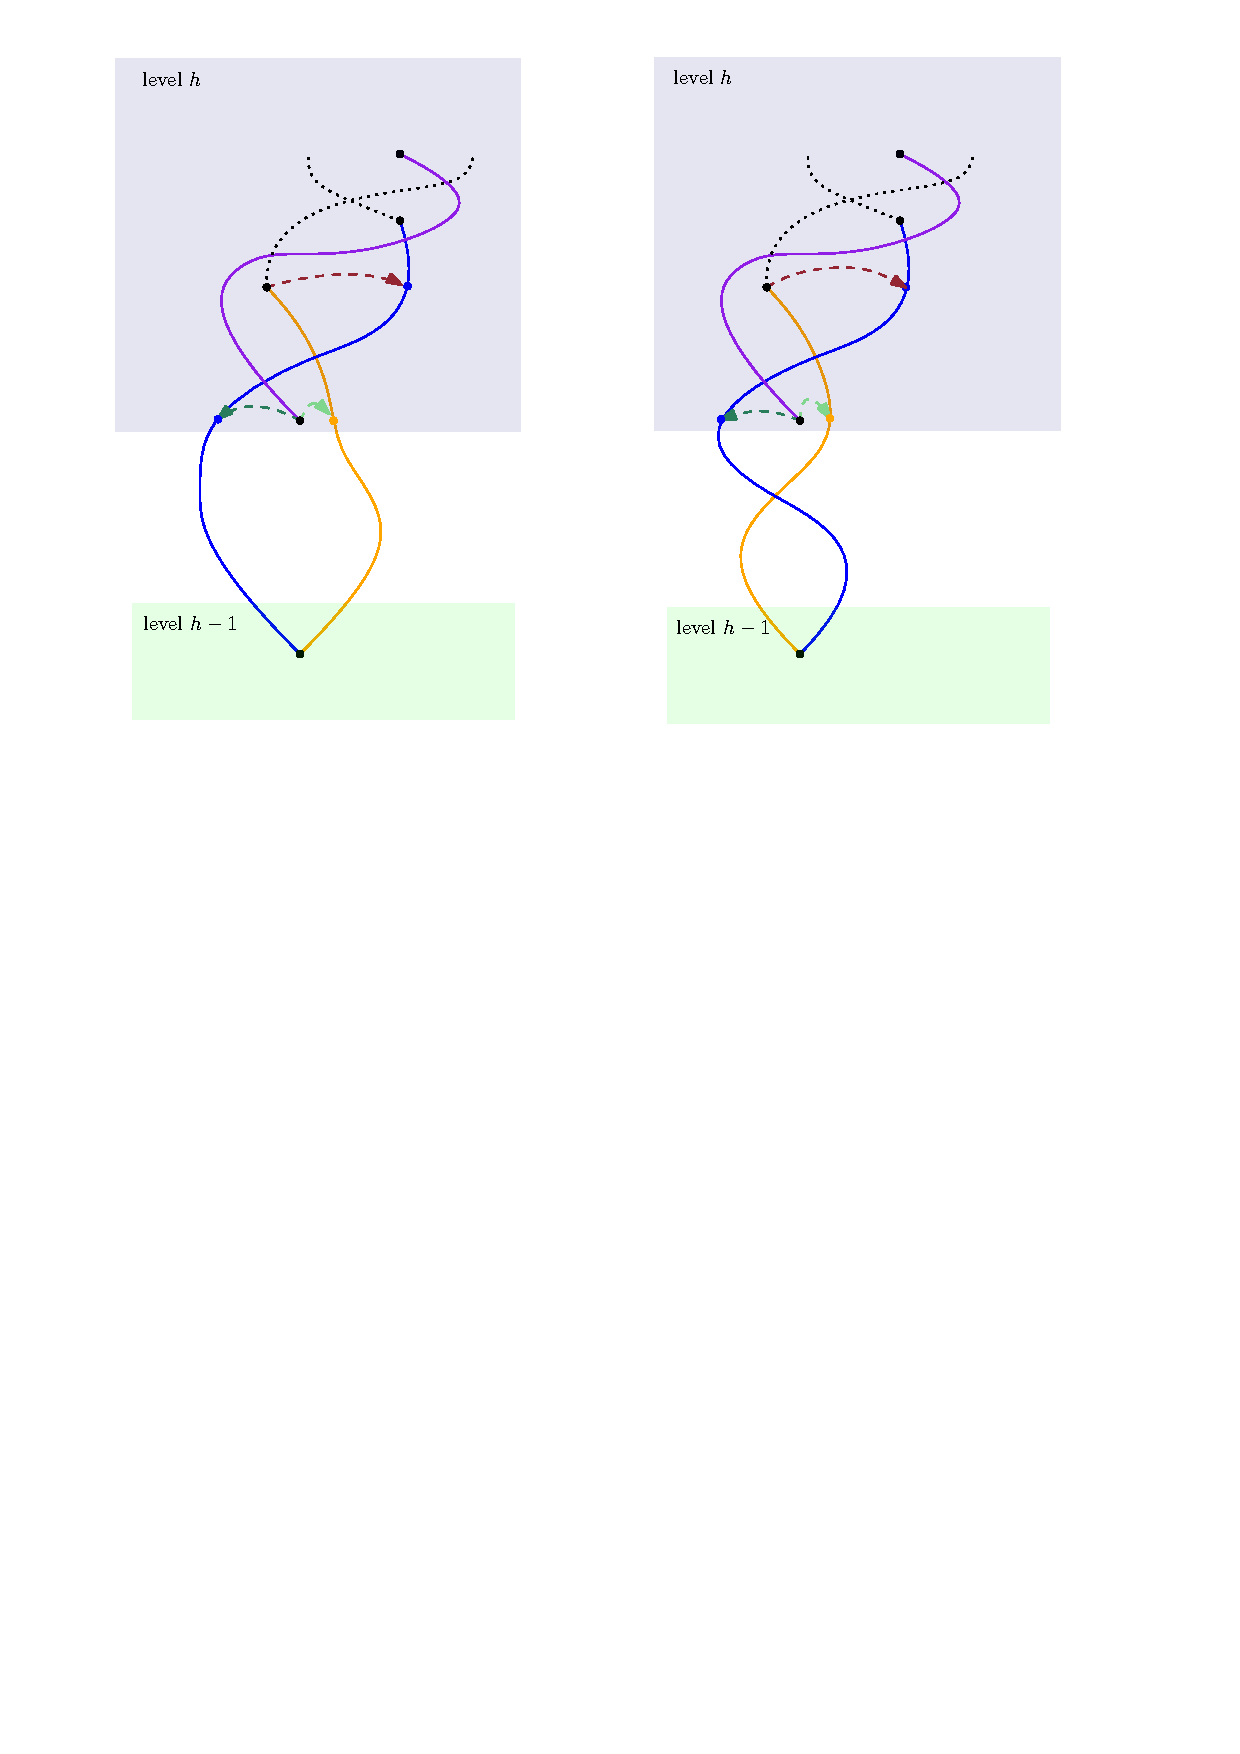
\includegraphics{figures/odd_cross_consecutive.pdf
}
\caption{consecutive edges in rotation that crosses oddly}
  \label{fig:occ}
\end{figure}
\begin{figure} [bt]
  \centering
  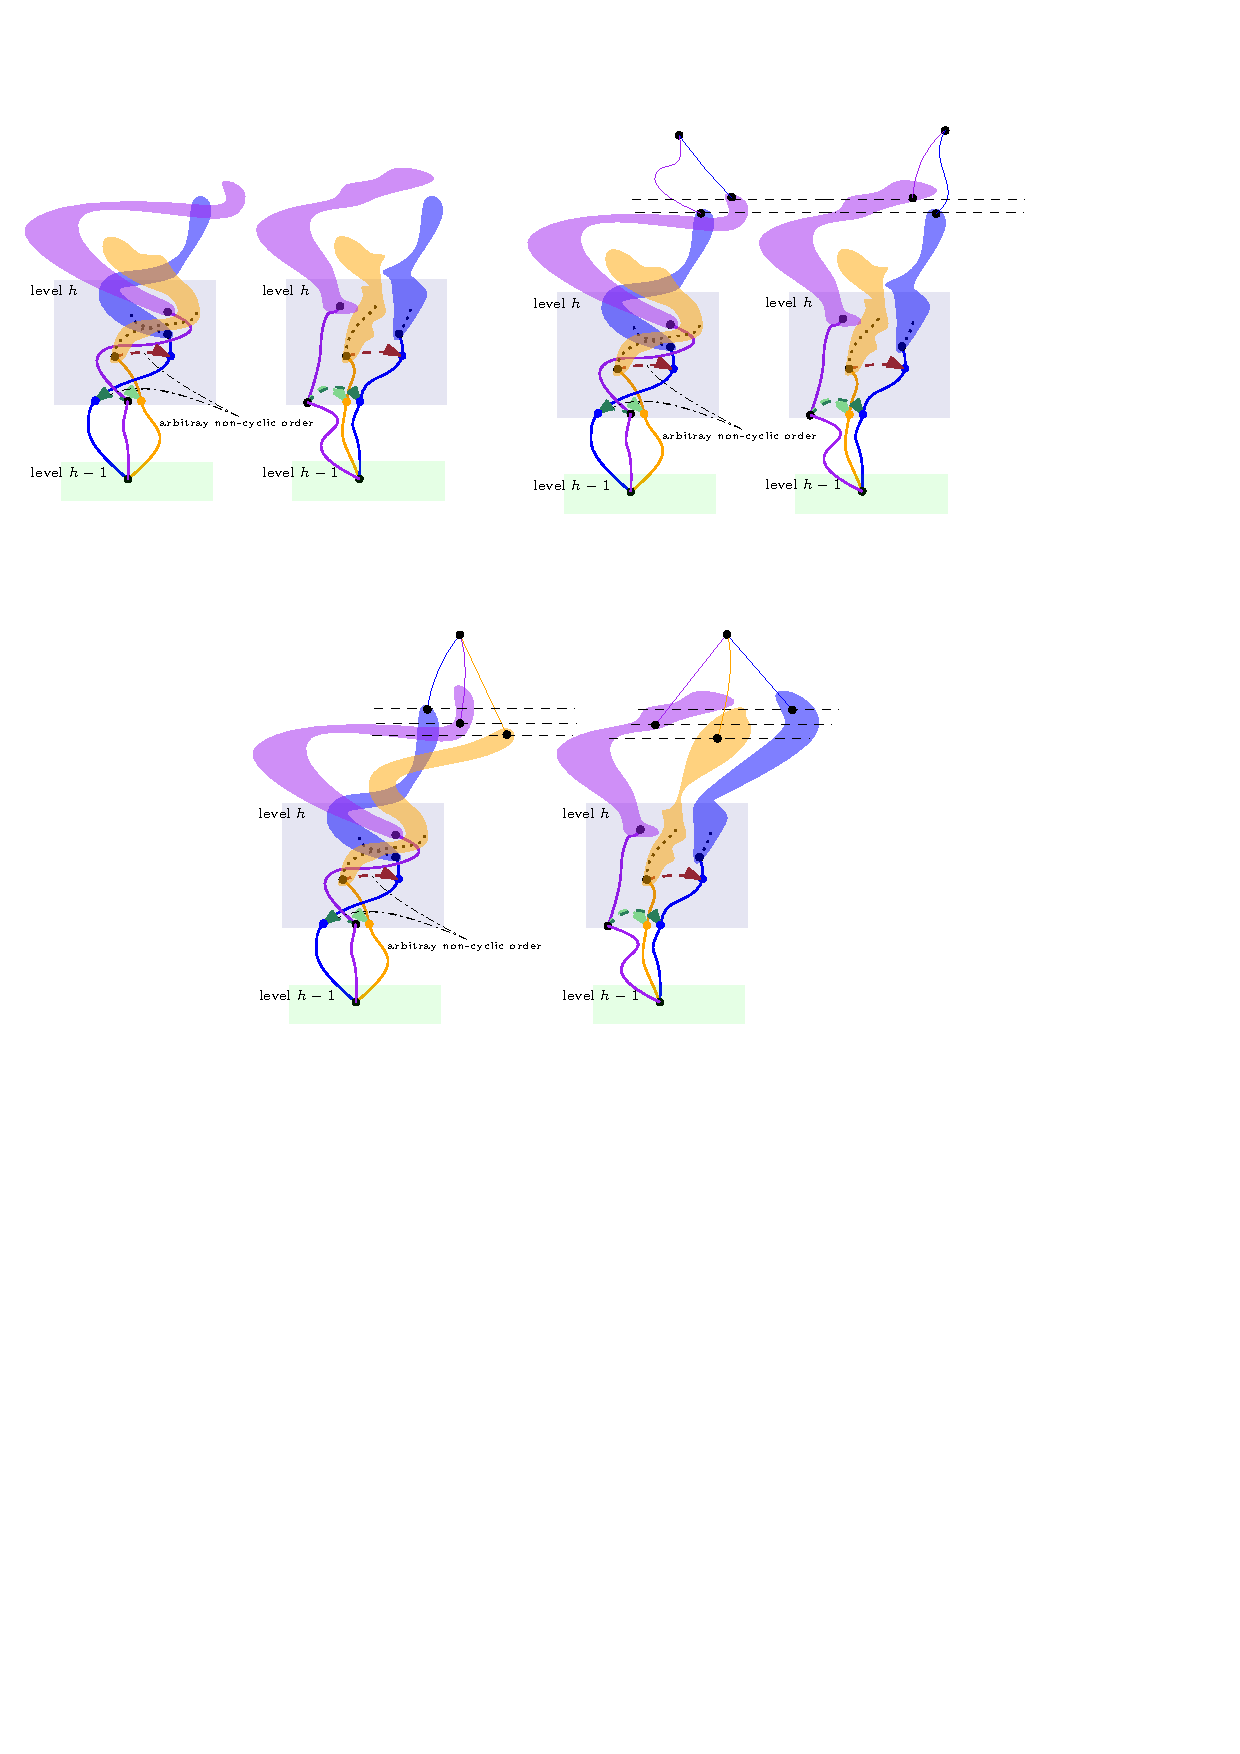
\includegraphics{figures/threecases_of_inbetweenvertex.pdf}
\caption{in between even crossing edge}
  \label{fig:toi}
\end{figure}
% basically i want to go throught the graph one vertex at a time, and construct the graph incrementely 
% when we find a vertex with adjacent edges we add restrictions on the equivalent classes. (basically we 
% propagate the order of the adjacent vertices to the vertices that can't get reached by relying just on planarity constraint)

%\begin{table} [bt]
%\centering
%\caption{Some strange numbers.}
%\begin{tabular}{rr}
%\toprule
%First column & Second column \\
%\midrule
%3\,109\,218\,136 & 3\,208\,415\,108 \\
%2\,231\,385\,058 & 1\,959\,477\,358 \\
%1\,287\,719\,872 & 1\,317\,165\,206 \\
%2\,516\,844\,936 & 2\,630\,583\,944 \\
%1\,569\,466\,774 & 1\,636\,507\,220 \\
%1\,032\,627\,816 &    991\,322\,491 \\
%\bottomrule
%\end{tabular}
%\label{tbl:randomnumbers}
%\end{table}
%
%\begin{figure} [bt]
%  \centering
%  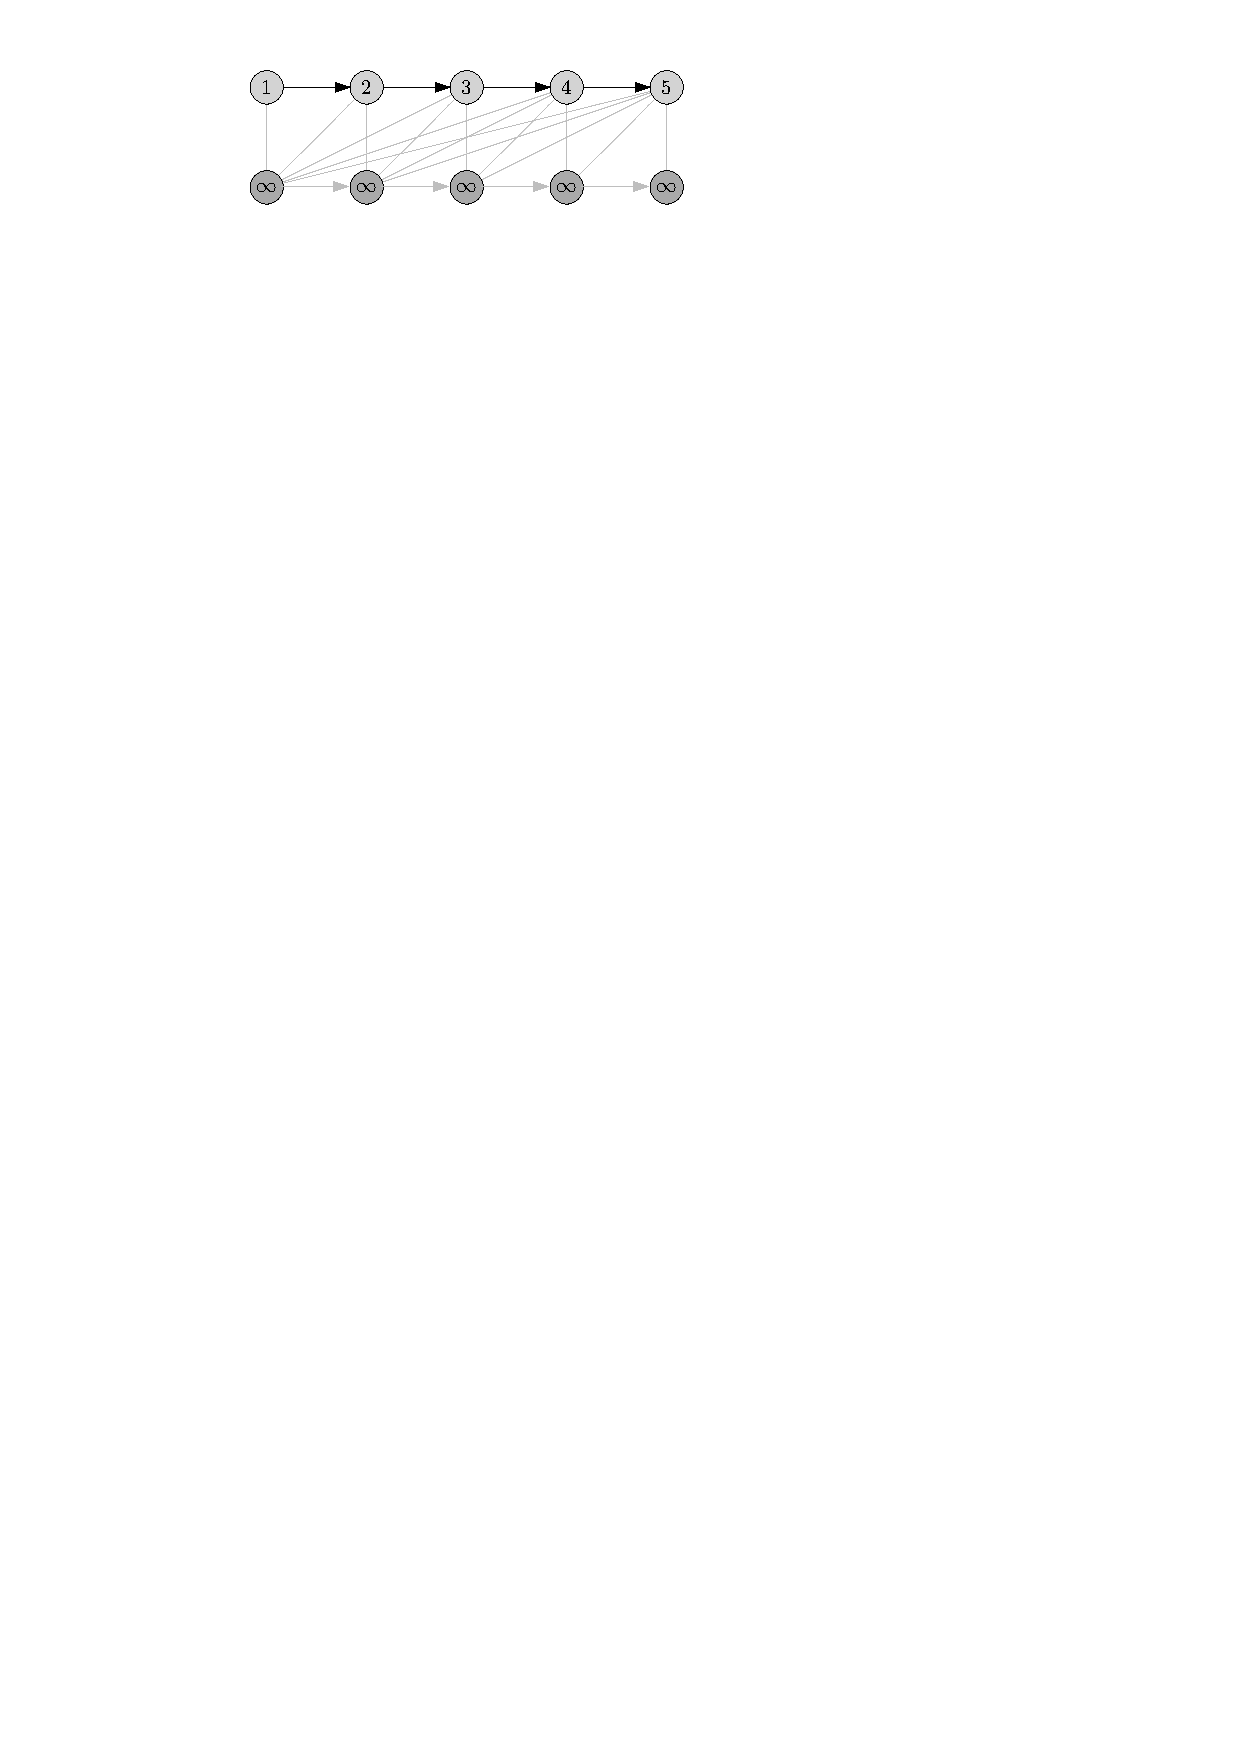
\includegraphics{figures/somegraph}
%  \caption{A funny graph.}
%  \label{fig:somegraph}
%\end{figure}
%
%

\include{conclusion}


%% --------------------
%% |   Bibliography   |
%% --------------------

\cleardoublepage
\phantomsection
\addcontentsline{toc}{chapter}{\bibname}

\iflanguage{english}
{\bibliographystyle{alpha}}
%{\bibliographystyle{babalpha-fl}} % german style

\bibliography{references}


%% ----------------
%% |   Appendix   |
%% ----------------

\cleardoublepage
\input{appendix}


\end{document}
